% !TEX root = ../BeamerTemplate.tex
%%%%%%%%%%%%%%%%%%%%%%%%%%%%%%%%%%%%%%%%%%%%%%%%%%%%%%%%%%%%%%%%%%%%%%%%%%%%%%%%%%

\section{Comparison of Hybrid, Sionna-RT, and SBR+}

\subsection{Comparison Basis}

\begin{frame}[t,shrink=8]{Three-Solver Comparison Framework}
    \begin{columns}[T,onlytextwidth]
        \begin{column}{0.52\textwidth}
            \begin{block}{Common comparison basis}
                \begin{itemize}
                    \item Same underlying antenna-lens geometry
                    \item Canonical $\mathrm{rx}1$--$\mathrm{rx}3$ and
                    $\mathrm{tx}1$--$\mathrm{tx}3$ ordering
                    \item Common frequencies: 37, 38, and 39~GHz
                    \item With-lens and without-lens conditions retained
                    \item Complex magnitude and phase used for MIMO evaluation
                \end{itemize}
            \end{block}
        \end{column}
        \begin{column}{0.44\textwidth}
            \begin{alertblock}{Required harmonization}
                HFSS Hybrid uses swept incident-angle excitations, whereas
                Sionna-RT and SBR+ use explicit transmitter indices.
            \end{alertblock}
            \begin{exampleblock}{Canonical mapping}
                The native antenna names are remapped into one common
                $3\times3$ channel convention before any solver-to-solver
                comparison is performed.
            \end{exampleblock}
        \end{column}
    \end{columns}
\end{frame}

\begin{frame}[t,shrink=20]{Raw and Normalized Comparisons Answer Different Questions}
    \begin{columns}[T,onlytextwidth]
        \begin{column}{0.47\textwidth}
            \begin{block}{Raw complex channel}
                \[
                    \mathbf H(f)
                \]
                Retains absolute propagation gain.

                \vspace{2mm}
                \textbf{Used for:}
                \begin{itemize}
                    \item Received channel magnitude
                    \item Absolute lens gain
                    \item Raw MIMO capacity
                \end{itemize}
            \end{block}
        \end{column}
        \begin{column}{0.49\textwidth}
            \begin{block}{Frobenius-normalized channel}
                \[
                    \widetilde{\mathbf H}
                    =\frac{\mathbf H}{\lVert\mathbf H\rVert_{\mathrm F}}
                \]
                Removes the overall channel-strength difference.

                \vspace{2mm}
                \textbf{Used for:}
                \begin{itemize}
                    \item Relative spatial-mode balance
                    \item Normalized singular values
                    \item Structural comparison across solvers
                \end{itemize}
            \end{block}
        \end{column}
    \end{columns}
    \begin{alertblock}{Interpretation rule}
        Raw and normalized results are complementary and must not be
        interpreted interchangeably.
    \end{alertblock}
\end{frame}

\subsection{Channel-Magnitude Agreement}

\begin{frame}[t,shrink=12]{Absolute Channel Magnitude: With Lens}
    \centering
    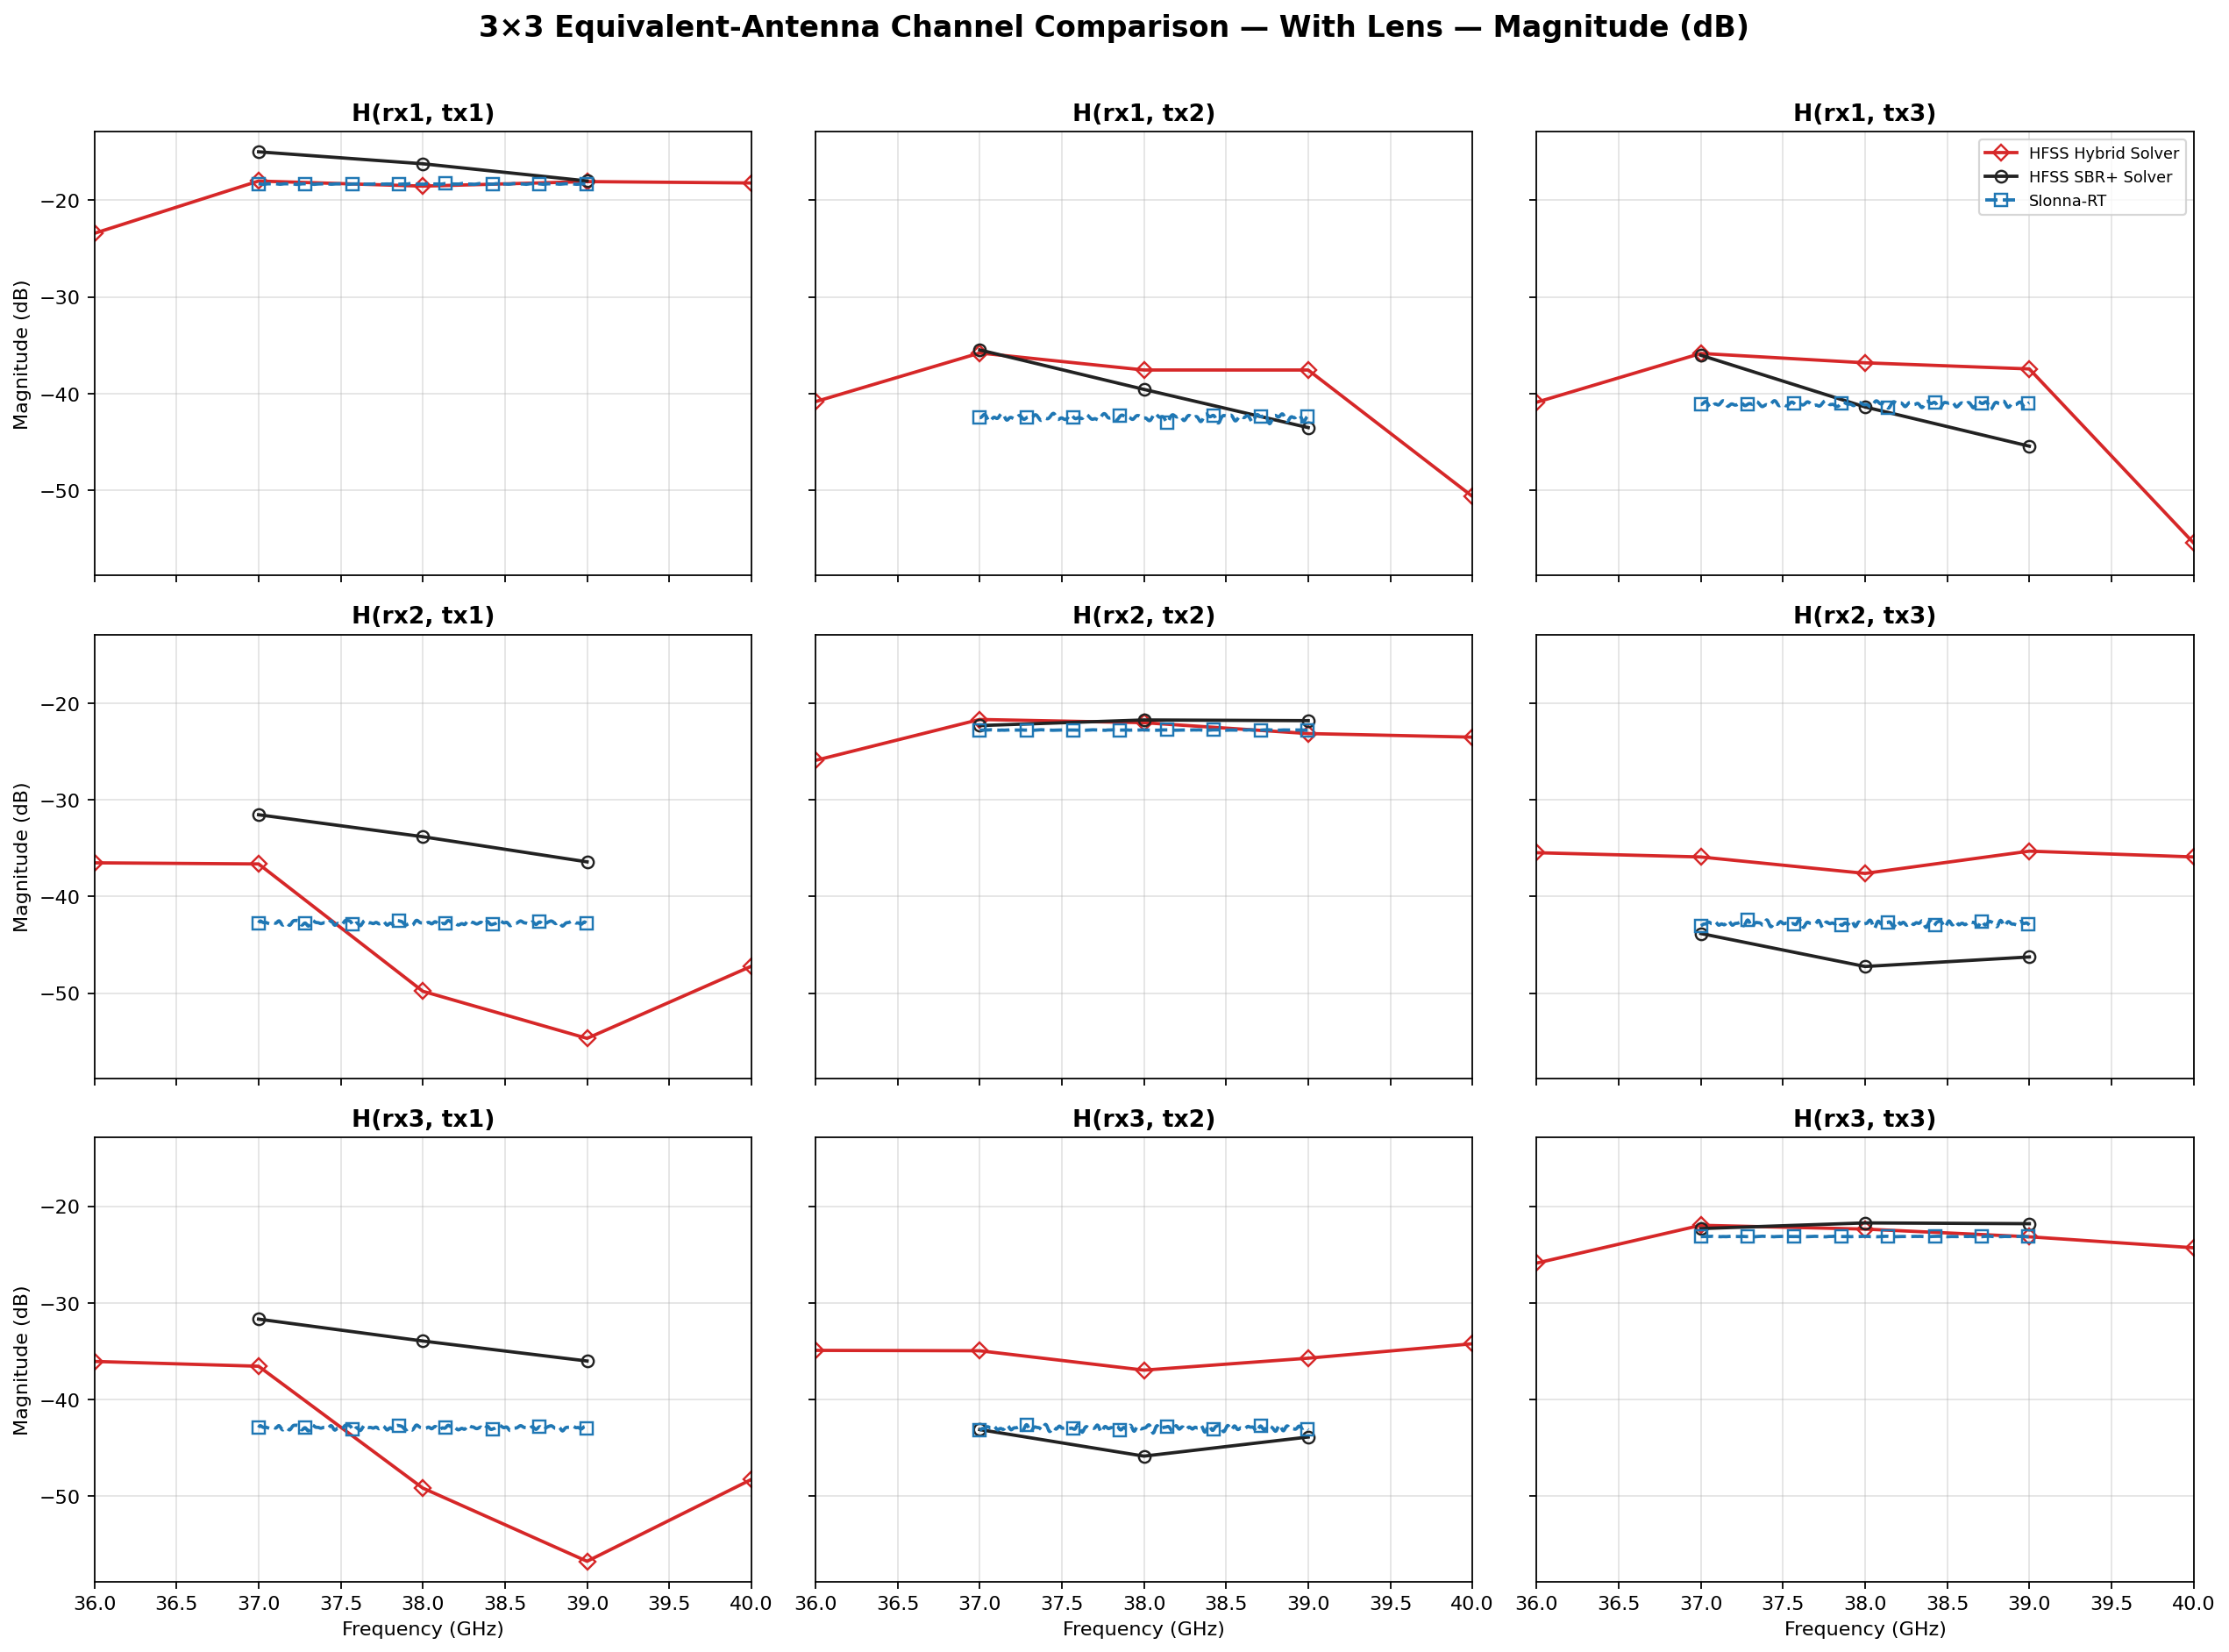
\includegraphics[width=\textwidth,height=0.73\textheight,keepaspectratio]
        {../current_report/image/channel_comparison_results/channel_3x3_with_magnitude_db.png}

    \begin{exampleblock}{Observation}
        \small
        All solvers reproduce the same broad channel organization, although
        the predicted absolute magnitudes remain solver-dependent.
    \end{exampleblock}
\end{frame}

\begin{frame}[t,shrink=15]{Absolute Channel Magnitude: Without Lens}
    \centering
    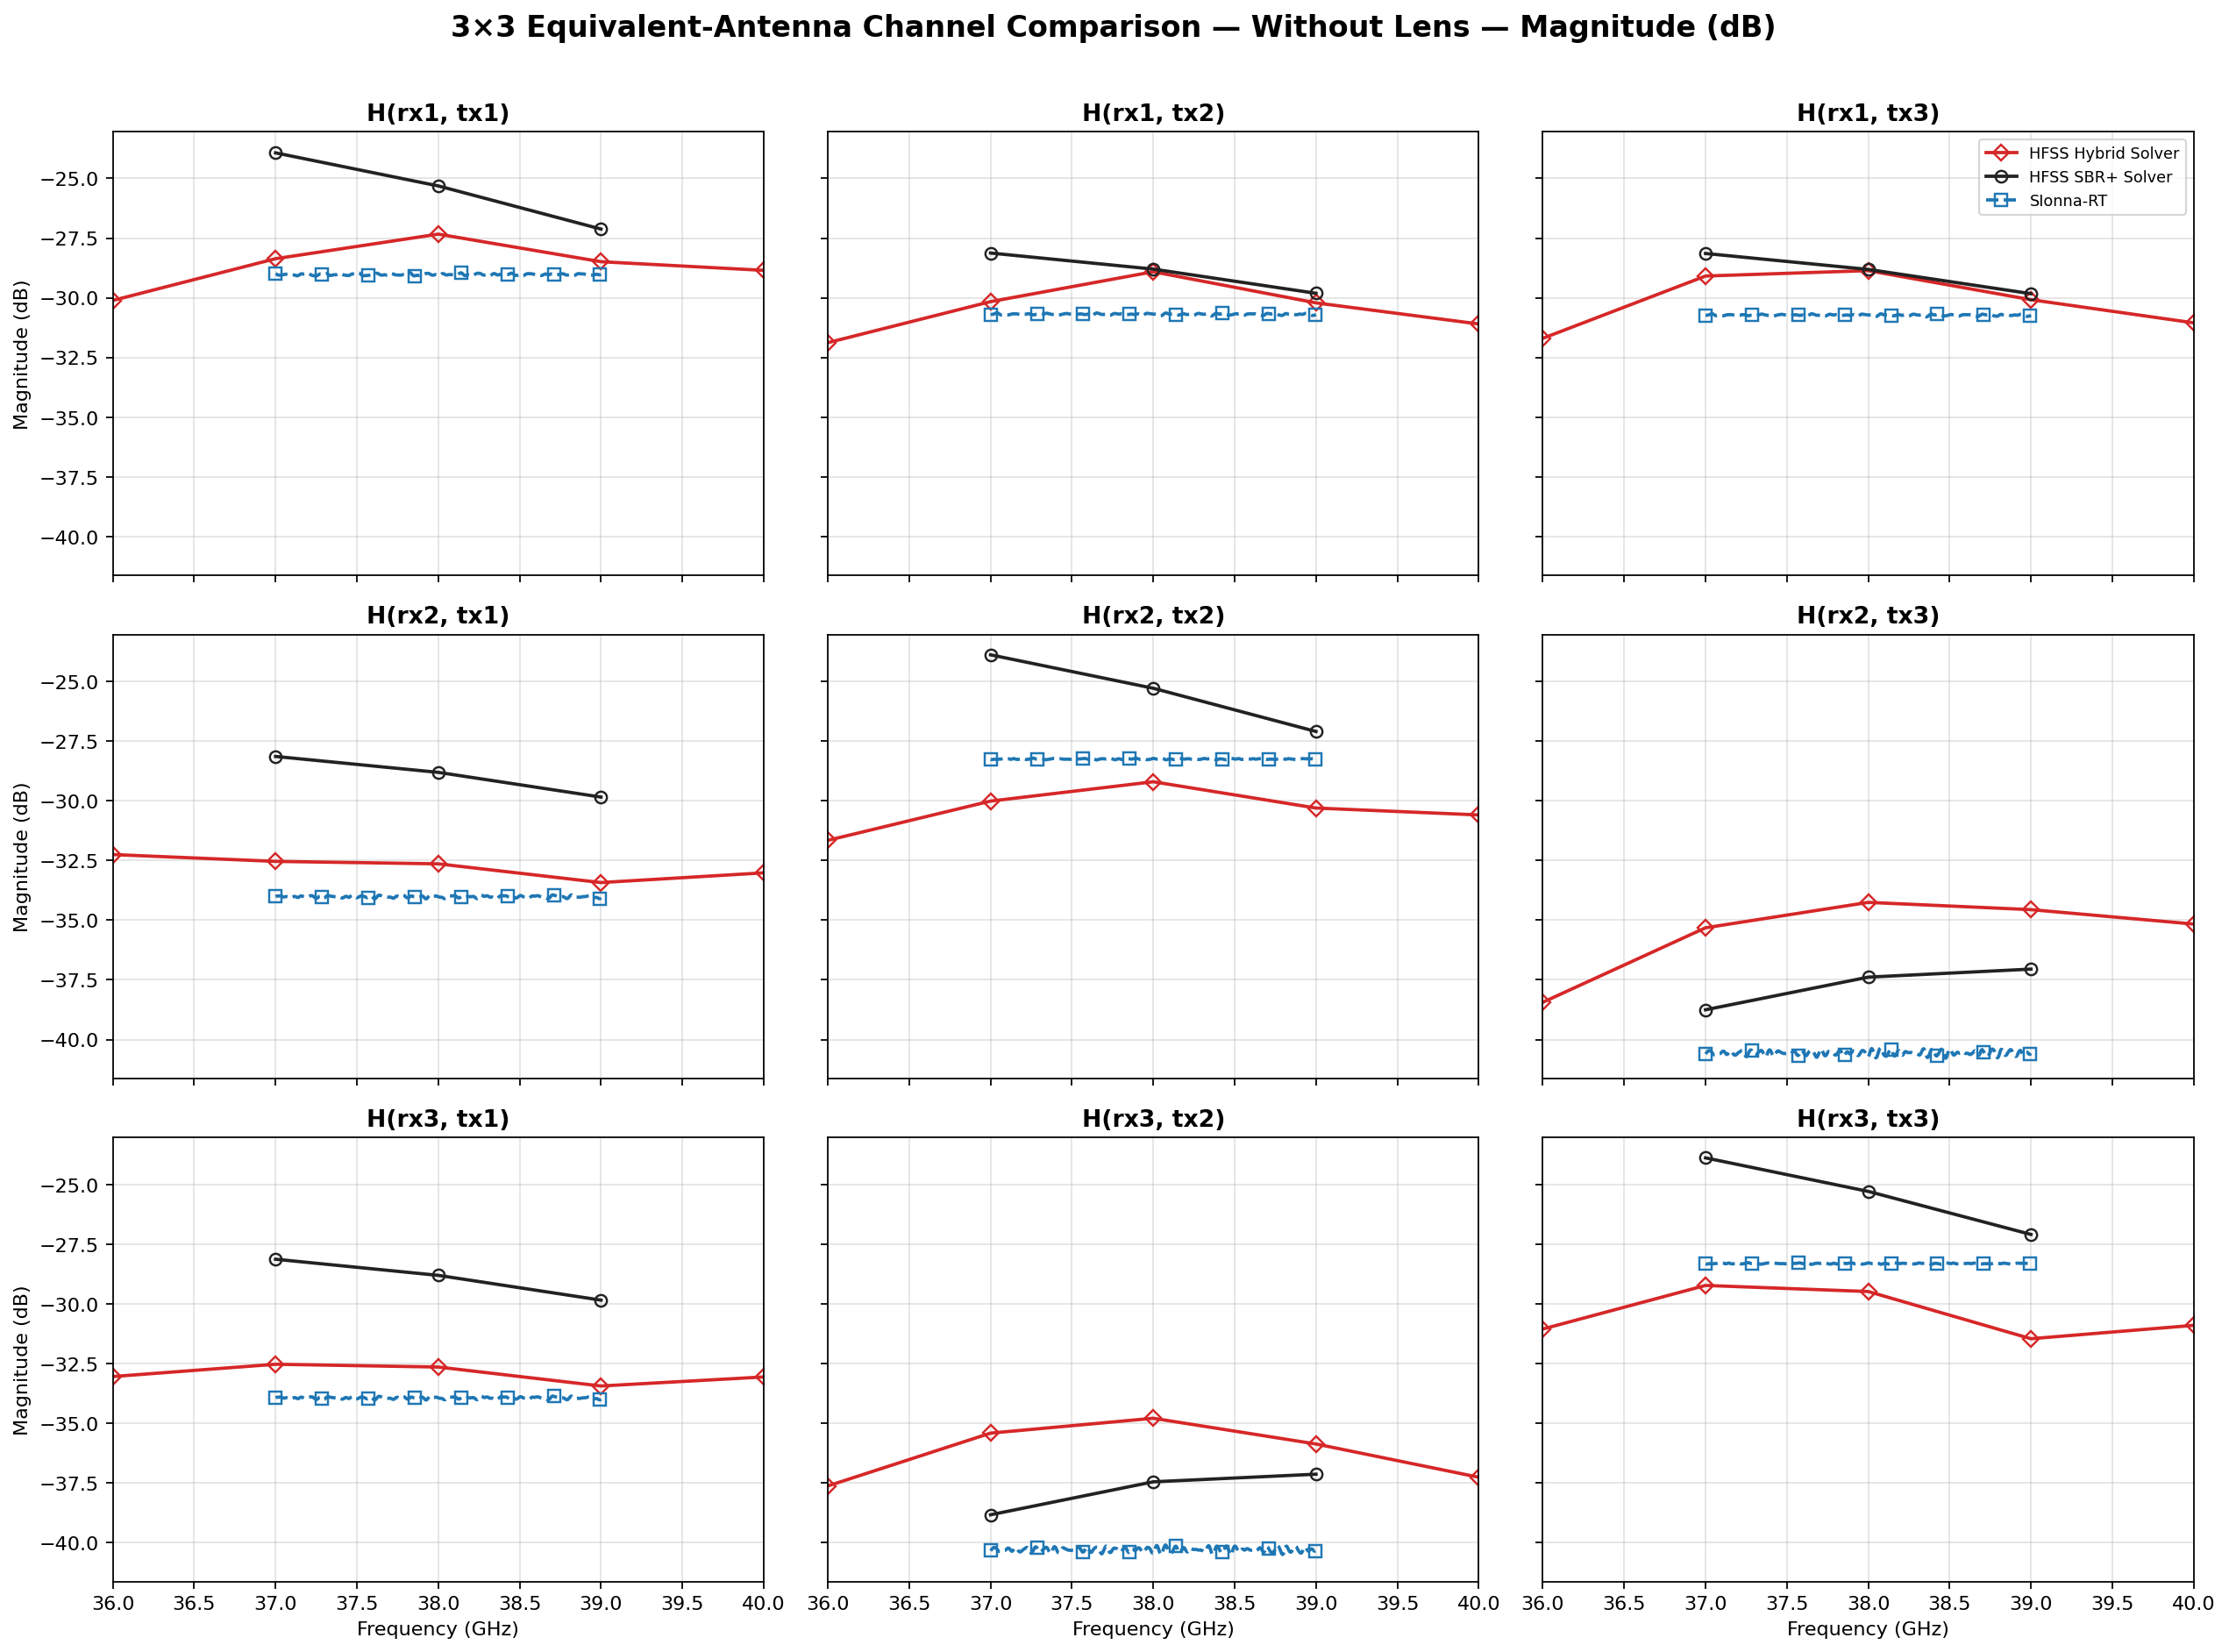
\includegraphics[width=\textwidth,height=0.73\textheight,keepaspectratio]
        {../current_report/image/channel_comparison_results/channel_3x3_without_magnitude_db.png}

    \begin{exampleblock}{Observation}
        \small
        The common spatial structure remains visible, but differences arise
        from field formulation, propagation approximation, antenna modeling,
        and channel extraction.
    \end{exampleblock}
\end{frame}

% \begin{frame}[t,shrink=10]{Pairwise Solver Discrepancy}
%     \begin{columns}[T,onlytextwidth]
%         \begin{column}{0.65\textwidth}
%             \centering
%             \includegraphics[width=\linewidth,height=0.72\textheight,keepaspectratio]
%                 {../current_report/image/channel_comparison_results/inter_solver_pairwise_discrepancy.png}
%         \end{column}
%         \begin{column}{0.32\textwidth}
%             \scriptsize
%             \begin{block}{With lens}
%                 Closest pair: \textbf{SBR+--Sionna-RT}
%                 \begin{itemize}
%                     \item Magnitude: 3.66~dB
%                     \item Centered shape: 1.46~dB
%                 \end{itemize}
%             \end{block}
%             \begin{block}{Without lens}
%                 Closest pair: \textbf{Hybrid--Sionna-RT}
%                 \begin{itemize}
%                     \item Magnitude: 2.20~dB
%                     \item Centered shape: 0.49~dB
%                 \end{itemize}
%             \end{block}
%             \begin{exampleblock}{Phase}
%                 Hybrid--SBR+ has the closest no-lens aligned phase:
%                 approximately $4.70^\circ$ mean difference.
%             \end{exampleblock}
%         \end{column}
%     \end{columns}
% \end{frame}

\subsection{Lens-Effect Agreement}

\begin{frame}[t,shrink=12]{Lens-Induced Change Across All Links}
    \begin{columns}[T,onlytextwidth]
        \begin{column}{0.68\textwidth}
            \centering
            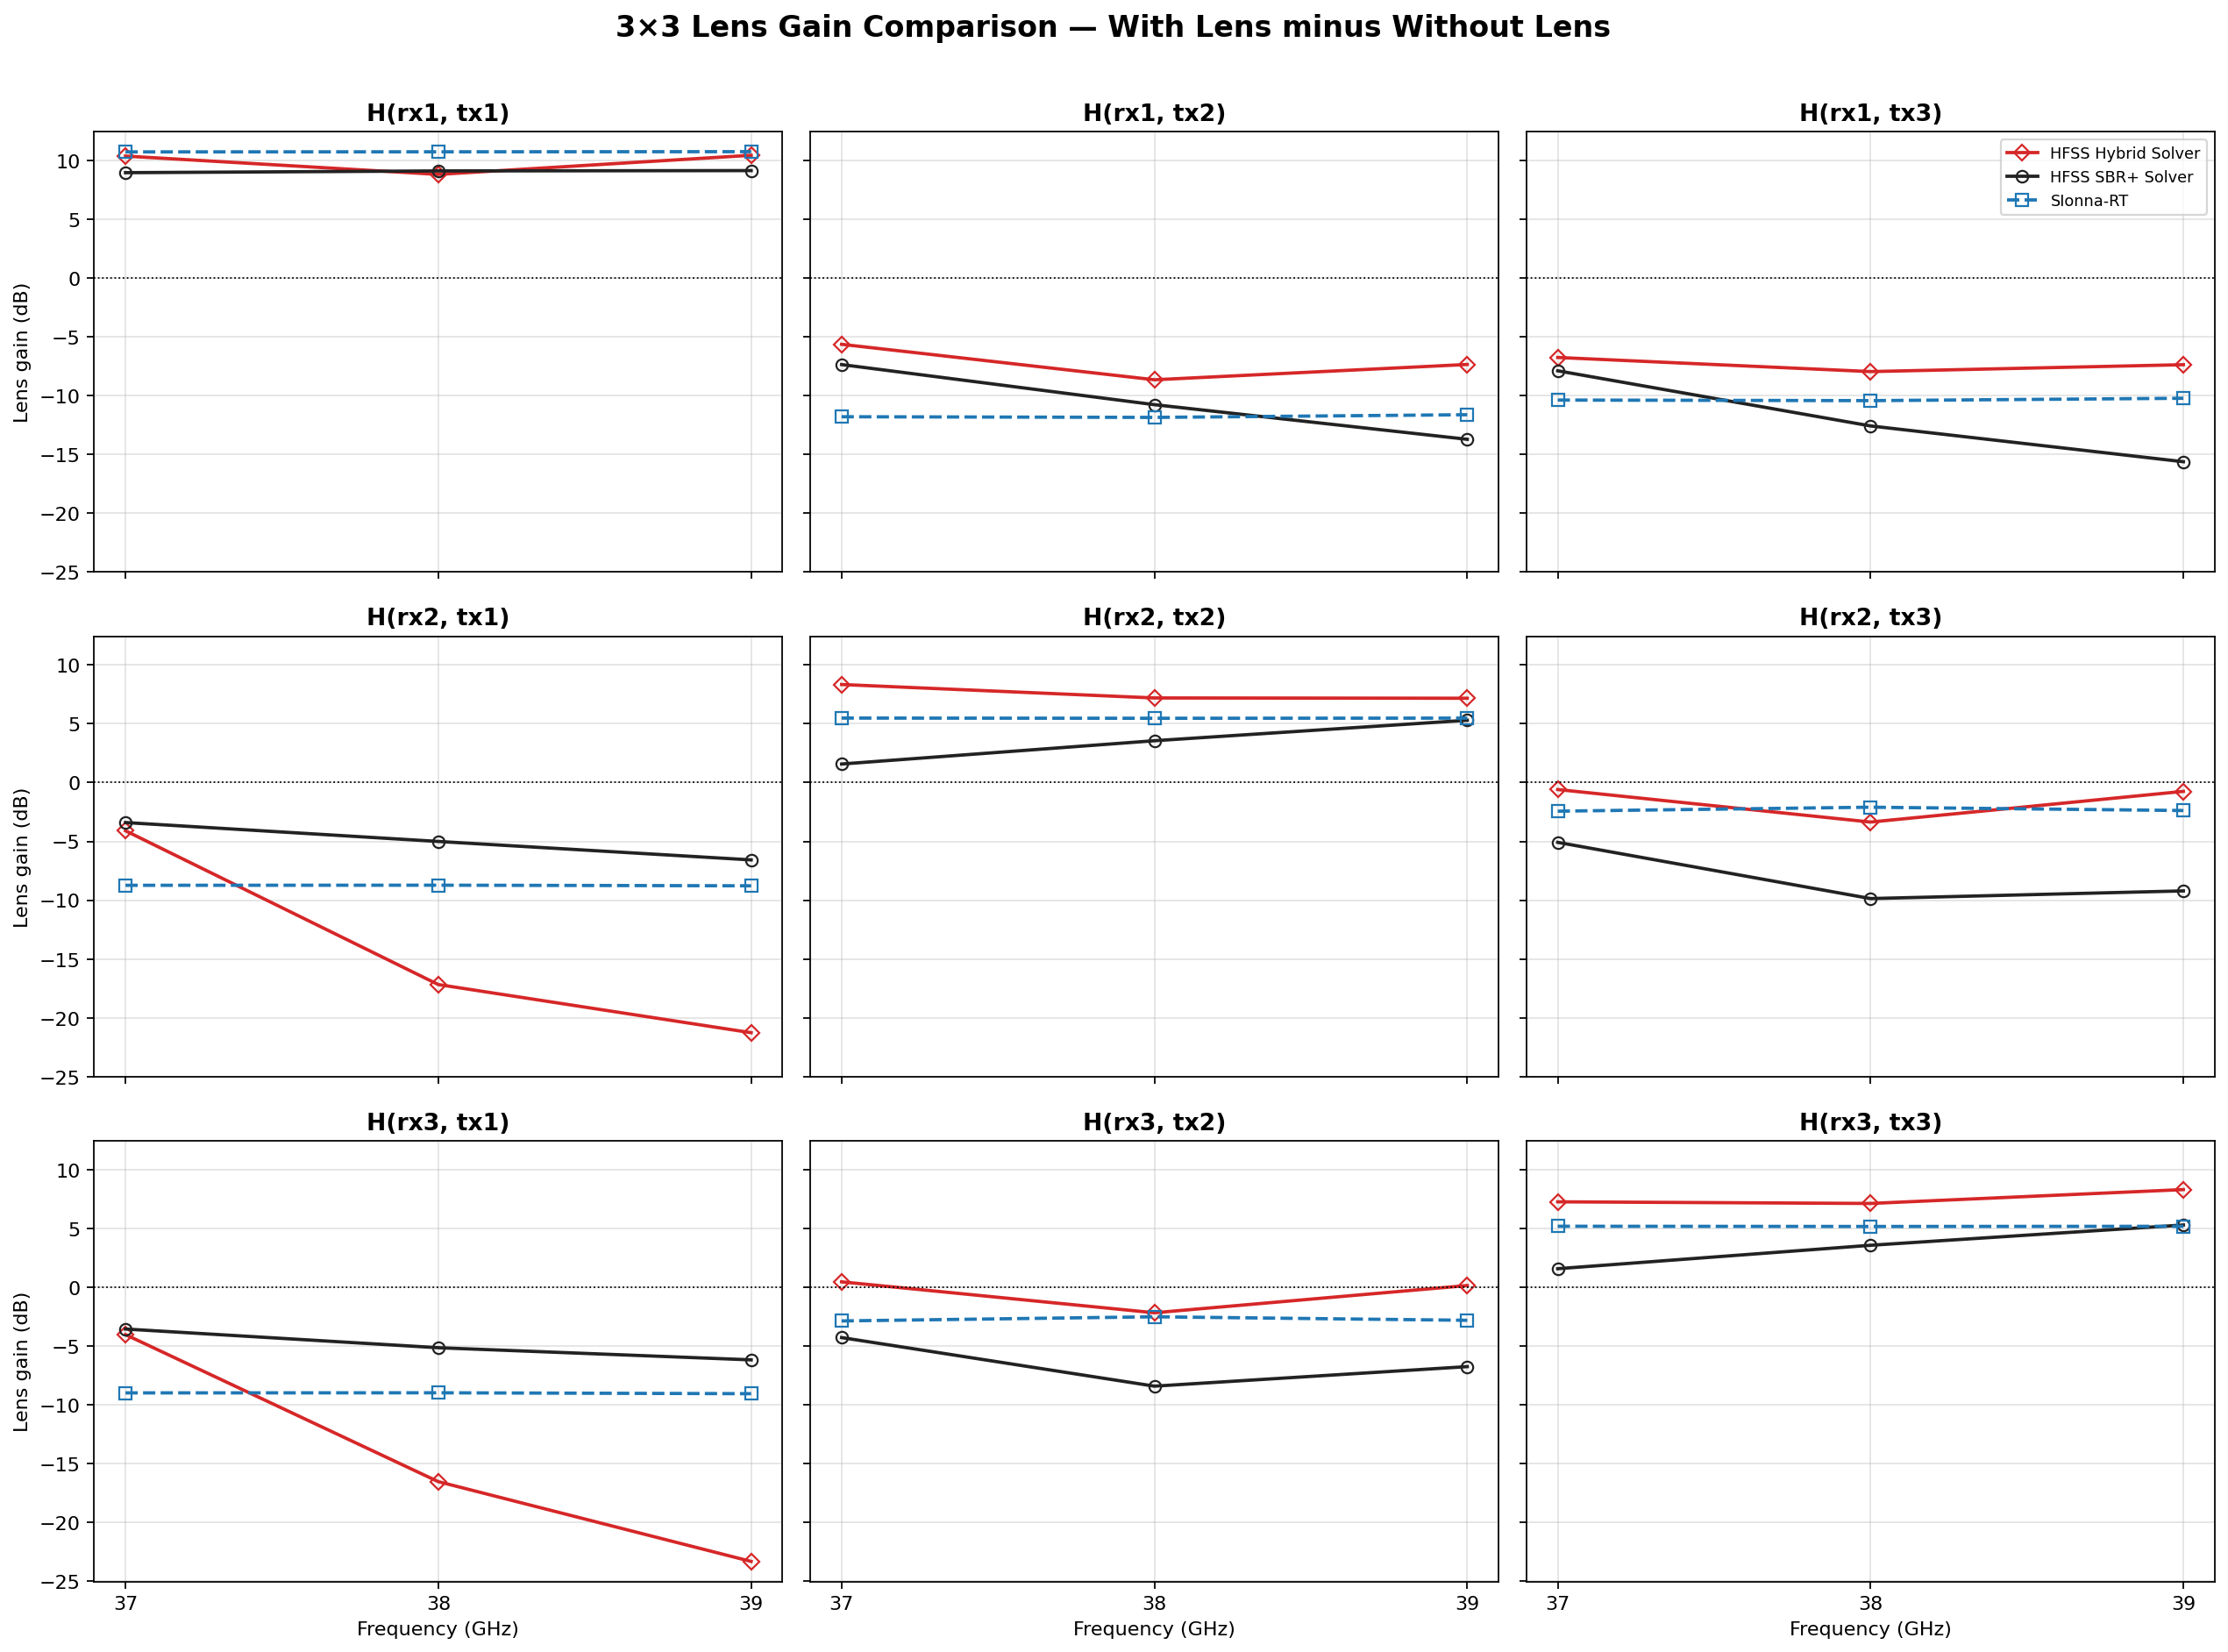
\includegraphics[width=\linewidth,height=0.73\textheight,keepaspectratio]
                {../current_report/image/channel_comparison_results/channel_3x3_lens_gain.png}
        \end{column}
        \begin{column}{0.29\textwidth}
            \scriptsize
            \[
                \Delta H_{\mathrm{lens}}
                =H_{\mathrm{with,dB}}-H_{\mathrm{without,dB}}
            \]
            \begin{block}{Mean diagonal gain}
                \begin{tabular}{@{}lr@{}}
                    Hybrid & $+8.33$~dB \\
                    SBR+ & $+5.33$~dB \\
                    Sionna-RT & $+7.12$~dB
                \end{tabular}
            \end{block}
            \begin{block}{Mean off-diagonal change}
                \begin{tabular}{@{}lr@{}}
                    Hybrid & $-7.58$~dB \\
                    SBR+ & $-7.86$~dB \\
                    Sionna-RT & $-7.48$~dB
                \end{tabular}
            \end{block}
        \end{column}
    \end{columns}
\end{frame}

\begin{frame}[t,shrink=18]{Agreement on the Direction of the Lens Effect}
    \begin{columns}[T,onlytextwidth]
        \begin{column}{0.58\textwidth}
            \centering
            
\includegraphics[width=\linewidth,height=0.67\textheight,keepaspectratio]
                {../current_report/image/channel_comparison_results/lens_effect_direction_agreement.png}
        \end{column}
        \begin{column}{0.38\textwidth}
            \begin{exampleblock}{Strong qualitative agreement}
                All three solvers agree on whether the lens increases or
                decreases magnitude at \textbf{25 of 27} link-frequency
                points:
                \[
                    \boxed{92.6\%}
                \]
            \end{exampleblock}
            \small
            The only non-unanimous cases are
            $H(\mathrm{rx}3,\mathrm{tx}2)$ at 37 and 39~GHz.

            \vspace{2mm}
            Exact gain differs, but the direction of the lens effect is highly
            consistent.
        \end{column}
    \end{columns}
\end{frame}

\subsection{MIMO Quality and Capacity}

\begin{frame}[t,shrink=12]{Raw-Channel MIMO Evaluation}
    \centering
    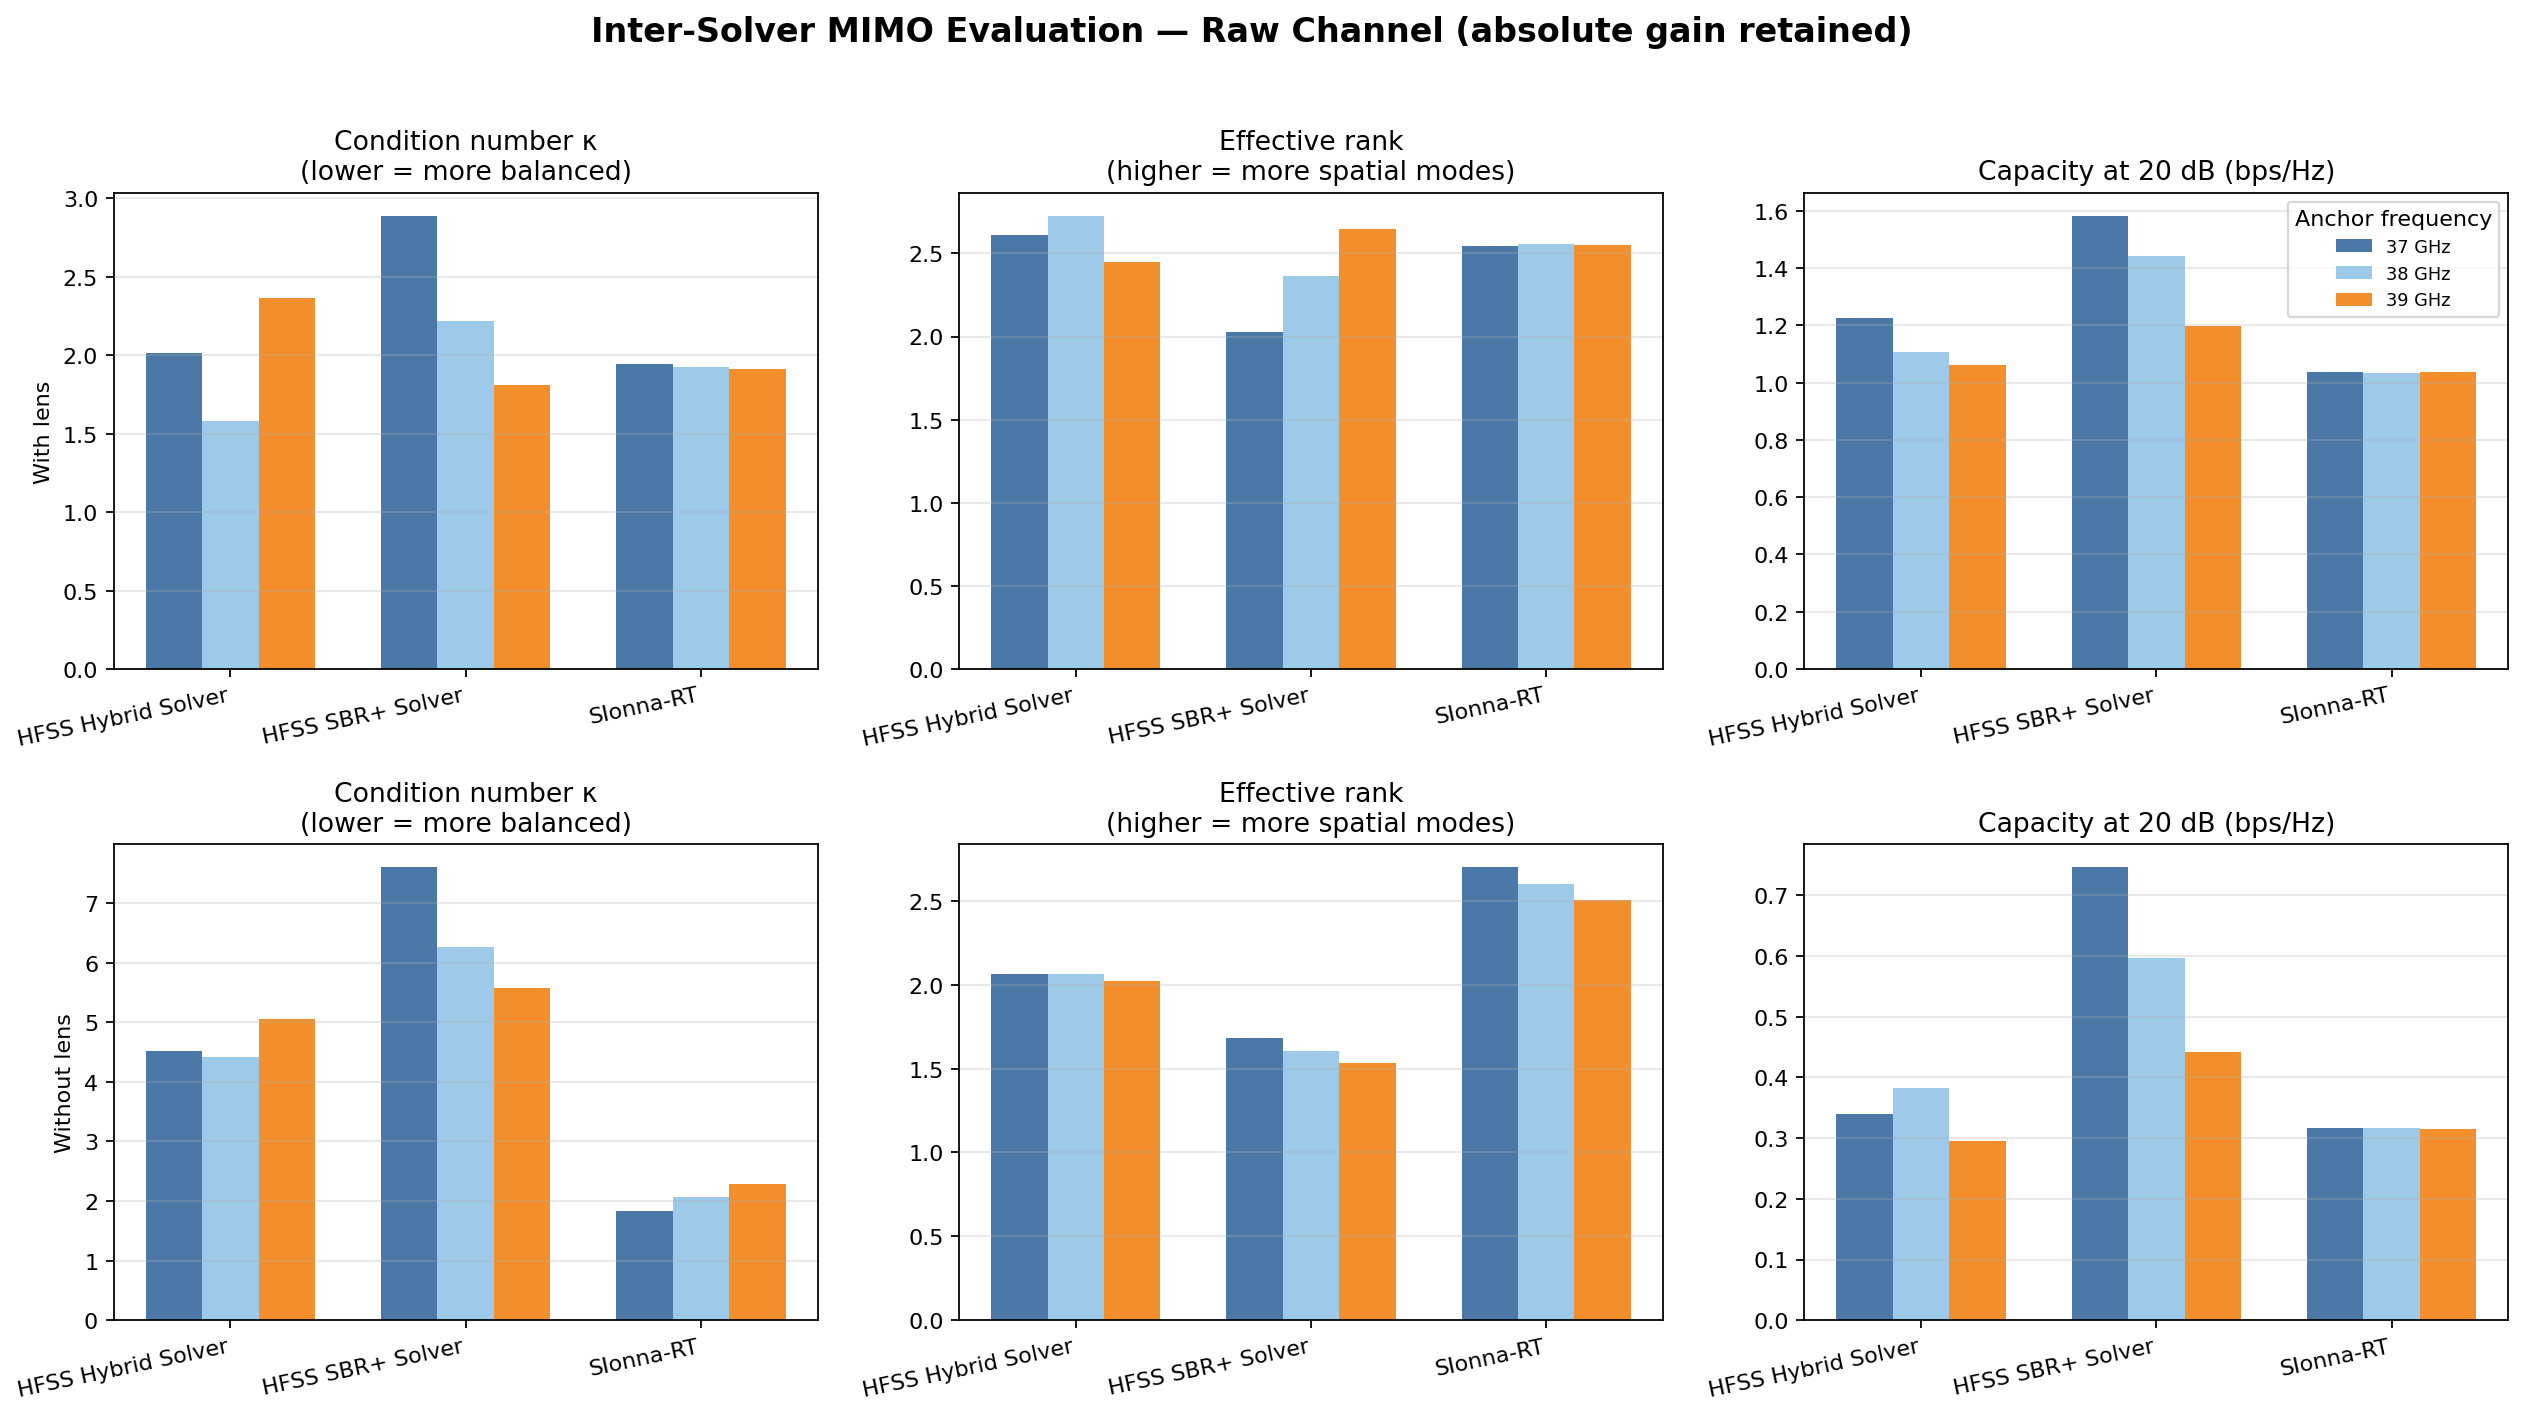
\includegraphics[width=\textwidth,height=0.73\textheight,keepaspectratio]
        {../current_report/image/channel_comparison_results/mimo_evaluation_raw.png}

    \begin{exampleblock}{Common result}
        \small
        At 38~GHz, every solver predicts higher raw 20-dB MIMO capacity after
        adding the lens.
    \end{exampleblock}
\end{frame}

\begin{frame}[t,shrink=8]{MIMO Metrics at 38~GHz}
    \centering
    \small
    \begin{tabular}{llrrr}
        \toprule
        \textbf{Solver} & \textbf{Lens} &
        \textbf{$\kappa$} & \textbf{$r_{\mathrm{eff}}$} &
        \makecell{\textbf{$C_{20\,\mathrm{dB}}$}\\\textbf{(bps/Hz)}} \\
        \midrule
        Hybrid    & With    & 1.579 & 2.728 & 1.108 \\
        Hybrid    & Without & 4.424 & 2.062 & 0.382 \\
        SBR+      & With    & 2.215 & 2.363 & 1.443 \\
        SBR+      & Without & 6.255 & 1.608 & 0.597 \\
        Sionna-RT & With    & 1.924 & 2.555 & 1.033 \\
        Sionna-RT & Without & 2.064 & 2.604 & 0.317 \\
        \bottomrule
    \end{tabular}

    \vspace{4mm}
    \begin{columns}[T,onlytextwidth]
        \begin{column}{0.31\textwidth}
            \begin{block}{Hybrid}
                Best with-lens balance:
                $\kappa=1.579$ and
                $r_{\mathrm{eff}}=2.728$.
            \end{block}
        \end{column}
        \begin{column}{0.31\textwidth}
            \begin{block}{SBR+}
                Highest raw capacity:
                $1.443$~bps/Hz.
            \end{block}
        \end{column}
        \begin{column}{0.31\textwidth}
            \begin{block}{Sionna-RT}
                Smallest condition-number change, but clear capacity gain from
                stronger modes.
            \end{block}
        \end{column}
    \end{columns}
\end{frame}

\begin{frame}[t,shrink=20]{Normalized Singular-Value Comparison}
    \begin{columns}[T,onlytextwidth]
        \begin{column}{0.68\textwidth}
            \centering
            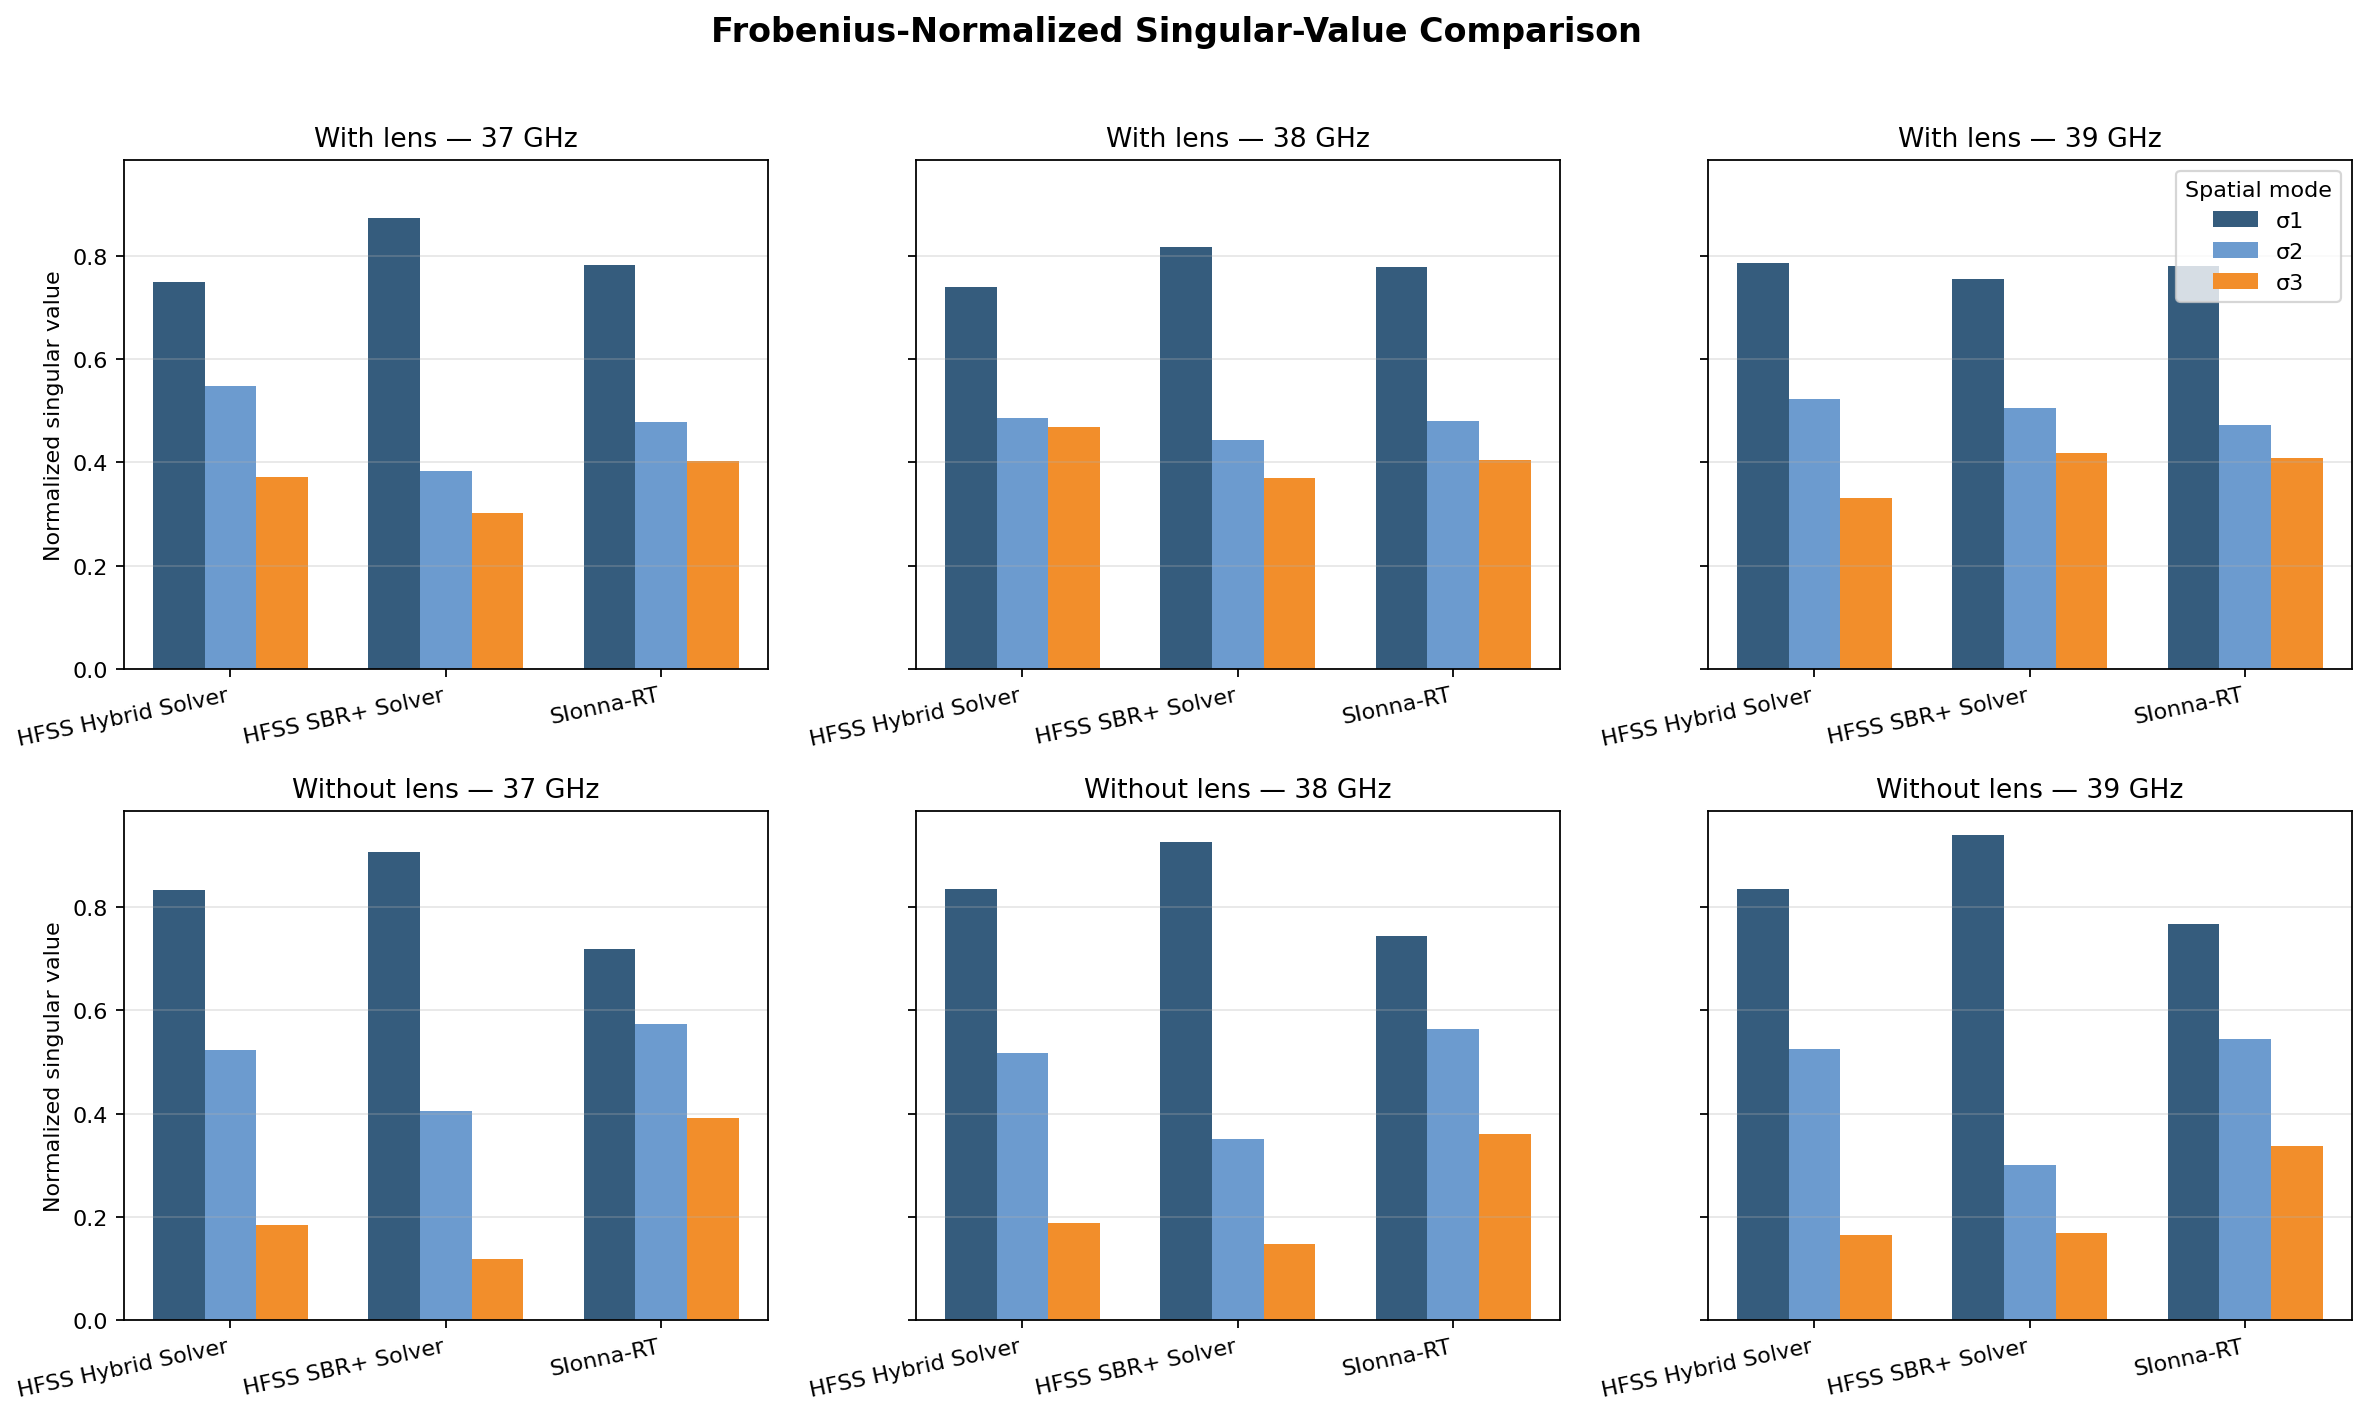
\includegraphics[width=\linewidth,height=0.73\textheight,keepaspectratio]
                {../current_report/image/channel_comparison_results/mimo_normalized_singular_values.png}
        \end{column}
        \begin{column}{0.29\textwidth}
            \small
            \begin{block}{With lens}
                All solvers retain three visible spatial modes at the anchor
                frequencies.
            \end{block}
            \begin{block}{Without lens}
                Hybrid and especially SBR+ show a relatively weak third mode;
                Sionna-RT predicts a more balanced normalized distribution.
            \end{block}
            \begin{alertblock}{Interpret jointly}
                Capacity rankings depend on both absolute strength and
                normalized spatial structure.
            \end{alertblock}
        \end{column}
    \end{columns}
\end{frame}

\subsection{Spatial Correlation}

\begin{frame}[t,shrink=12]{Inter-Solver Spatial-Correlation Comparison}
    \begin{columns}[T,onlytextwidth]
        \begin{column}{0.67\textwidth}
            \centering
            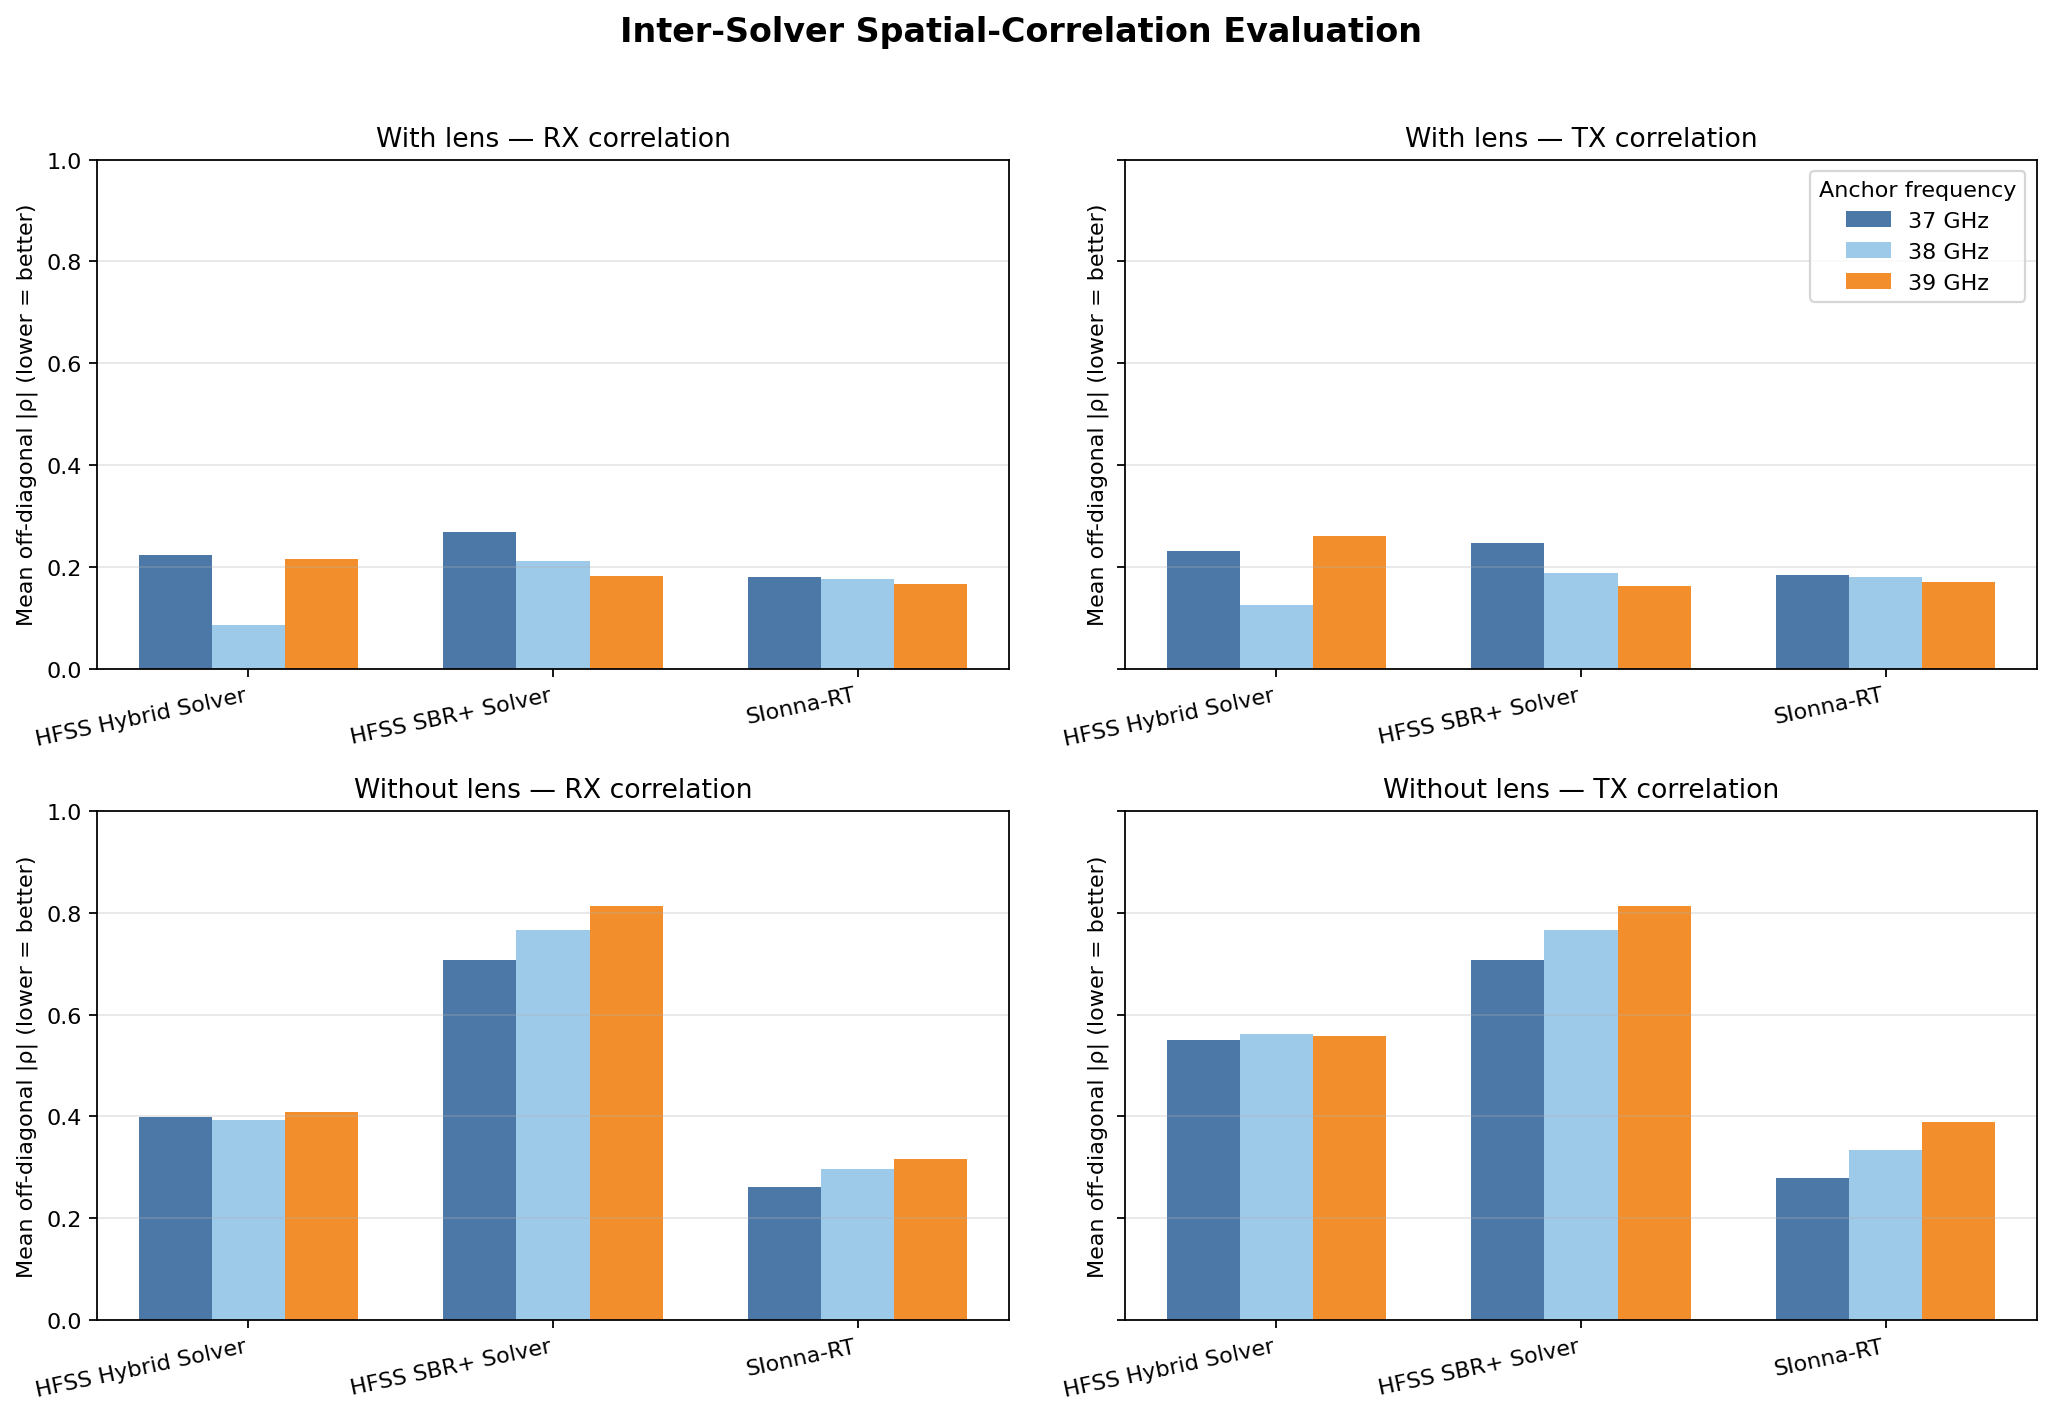
\includegraphics[width=\linewidth,height=0.73\textheight,keepaspectratio]
                {../current_report/image/channel_comparison_results/mimo_spatial_correlation_evaluation.png}
        \end{column}
        \begin{column}{0.30\textwidth}
            \scriptsize
            \begin{block}{38-GHz mean RX/TX correlation}
                \begin{tabular}{@{}lcc@{}}
                    \toprule
                    & \textbf{Lens} & \textbf{No lens} \\
                    \midrule
                    Hybrid & .085/.126 & .393/.561 \\
                    SBR+ & .213/.188 & .767/.767 \\
                    Sionna & .177/.181 & .297/.335 \\
                    \bottomrule
                \end{tabular}
            \end{block}
            \begin{exampleblock}{Unanimous result}
                Every solver predicts lower RX- and TX-side spatial
                correlation after adding the lens.
            \end{exampleblock}
        \end{column}
    \end{columns}
\end{frame}

\subsection{Overall Interpretation}

\begin{frame}[t,shrink=20]{What All Three Solvers Agree On}
    \begin{columns}[T,onlytextwidth]
        \begin{column}{0.49\textwidth}
            \begin{exampleblock}{Robust engineering conclusions}
                The antenna lens:
                \begin{itemize}
                    \item Reinforces direction-matched channels
                    \item Suppresses most cross-directional coupling
                    \item Increases raw 20-dB MIMO capacity
                    \item Reduces spatial correlation
                \end{itemize}
            \end{exampleblock}
        \end{column}
        \begin{column}{0.47\textwidth}
            \begin{block}{Solver-specific strengths}
                \begin{itemize}
                    \item \textbf{Hybrid:} best with-lens spatial balance at
                    38~GHz
                    \item \textbf{SBR+:} highest raw capacity
                    \item \textbf{Sionna-RT:} most stable full-band behavior
                \end{itemize}
            \end{block}
        \end{column}
    \end{columns}
    \begin{alertblock}{Boundary of the evidence}
        Agreement is strongest for qualitative lens trends and relative MIMO
        improvement. Exact magnitude and phase remain solver-specific until
        reconciled against measurement.
    \end{alertblock}
\end{frame}
